\documentclass[10pt]{article}
\usepackage[utf8]{inputenc}

\usepackage{geometry}
\usepackage{graphicx}

\geometry{portrait, margin=1.5in}

\begin{document}


\section{Exercise 1 - The Core}

 \subsection{Exercise 1.1}

During this exercise, responsibility driven design was followed, starting with the requirements.\\
The first classes that were considered as candidate classes were the following:
\begin{itemize}
  \item Game
  \item Alien
  \item Aliengrid
  \item SpaceShip
  \item EnemyBullet
\item Bullet
\item MovementController
\item PlayerBullet
\item Barricades
\item Powerup
\item Soundcontroller
\item Explosion
\item EnemyController
\item SpaceshipController
\item Main
\item Player
\item UI
\item UIController
\item Bulletcontroller

\end{itemize}

 \pagebreak
For this candidate classes CRC cards were made and these were distributed to the team. \\
By walking through scenarios unneeded and missing classes and responsibilities were uncovered.\\
Finally the following list of classes with their responsibilities and collaborations is created:
\begin{center}
    \begin{tabular}{ | p{3cm} | p{5cm} | p{3cm} | p{2cm} | p{2cm} |}
  \hline
    Class & Responsibility & Collaborates with & Super & Sub \\ \hline
   Game & All units in the game & all the controllers & & \\ \hline
   SpaceShipController & Activities of the spaceship & Game & & \\ \hline
  SpaceShip & Shooting a bullet & SpaceShipController & Unit & \\ \hline
  ShipBullet& & bulletController & Bullet & \\ \hline
   Player & The score and lives of the player & Game & & \\ \hline
  AlienController & The movements of the aliens & Game & &  \\  \hline
   Alien & Shooting a bullet  & AlienController & Unit &  \\  \hline
   AlienBullet & & Bullet & Bullet &  \\  \hline
   BulletController & Movements of the bullets & Game & &  \\  \hline
   Bullet & &  BulletController & Unit & AlienBullet ShipBullet \\  \hline
   ExplosionController & The development of the explosions & Game & &  \\  \hline
  Explosion & Counter of the explosion & ExplosionController & Unit &  \\  \hline
  BarricadeController & The changes of the barricades & Game & &  \\  \hline
  Barricade & Health of the barricade & BarricadeController & Unit &  \\  \hline
  Unit & Location, seize and speed of a unit &  & & Alien, Explosion, Barricade, Bullet, SpaceShip  \\  \hline
  Collisions & The collisions between all types of units  & Game & &  \\  \hline
  Draw  & The drawings of elements on the screen & SpaceInvadersUI & &  \\  \hline
  Drawbarricade & The drawings of the barricades & Draw & &  \\  \hline
  DrawBullet & The drawings of the bullets & draw & &  \\  \hline
  DrawSpaceShip & The drawings of the spaceship & draw & &  \\  \hline
  DrawAlien  & The drawings of the aliens & & &  \\  \hline
  SpaceInvadersUI & The presentation of the game on the screen & GameUIController & &  \\  \hline
  GameUIController & The keyboard inputs and refreshing the frames & SpaceInvadersUI & &  \\  \hline
  Main & The launch of the game & Game, GameUIController & &  \\  \hline
    \end{tabular}
\end{center}

The main difference with the actual implementation is that that game and gamUIController in the actual implementation have much more responsibilities.\\
It would have been better if these classes were split to smaller classes as in the responsibility driven design of classes as above. Because then it will be easier to make changes to the code while it is possible to just replace a small class without changing a very big class. \\
Classes that could be add to do this are the draw and control classes. 

 \pagebreak

 \subsection{Exercise 1.2}
The main classes implemented in the actual implementation are the game and gameUIController.
The game class has the responsibility to handle the movements of the spaceship and the bullets, the creation of barricades and to monitor the game status.\\
 This class also handles the lists of all the units in the game. It collaborates with the aliencontroller, collisions and player class. \\
Another main class implemented in the actual implementation is the GameUIController which deals with the drawings of all the elements and animation, loading of the sprites, creation of a new game,  and the key inputs.
 This class collaborates with the game and SpaceInvadersUI classes.\\


 \subsection{Exercise 1.3} 
Some of the classes are less important as the classes mentioned in previous exercise, because they has less responsibilities and could easier be merged with some other class.\\
They are also a lot smaller what makes it easier to merge them in another class. For example we have a ShipBullet and a AlienBullet class which are subclasses of the Bullet class. \\
 The ShipBullet and AlienBullet class could have been merged together in the bullet class. \\
The reason this is not done and we have shipbullet and alienbullet as separate classes, is because the product is still under development. \\
It is now possible to check with instance of if a bullet is a ship or an alien bullet. \\
With this construction it is also easier to add attributes or methods to the alien or ship bullet only.\\
 \pagebreak

 \subsection{Exercise 1.4} 
\begin{figure}[ht!]
\centering
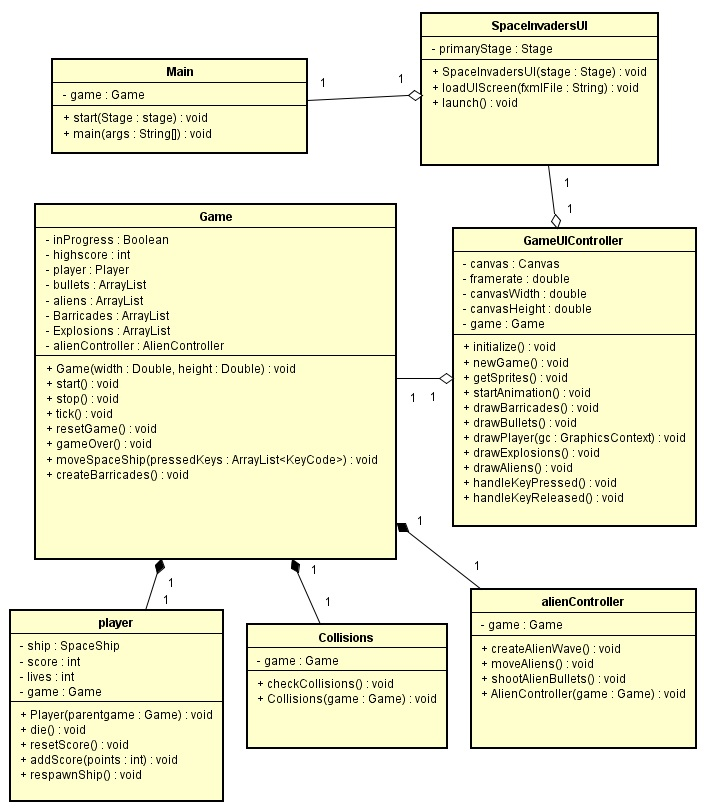
\includegraphics[width=14cm, height=16cm]{UMLSEM.jpg}
\end{figure}


\end{document}